\section{深度神经网络}
\frame
{
	\frametitle{\secname~ }
	\begin{block}{前馈神经网络}
		传统的人工神经网络
	\end{block}
	\begin{block}{卷积神经网络}
		目前最为流行的,广泛应用于视觉任务的神经网络
	\end{block}
	\begin{block}{长短记忆网络}
		与卷积网络相比,更适用于处理时序信号
	\end{block}
}
\subsection*{深度神经网络}
\frame{
	\frametitle{前馈神经网络结构}
	\begin{columns}[onlytextwidth]
		\begin{column}{0.5\textwidth}
			\vspace{-1.5em}
			\begin{itemize}
				\item 有向无环图的结构
				\item 输入层(数据特征)
				\item 隐含层(映射后的特征)
				\item 输出层(预测结果)
				\item 反向传播算法(训练方法)
			\end{itemize}
		\end{column}
		\begin{column}{0.5\textwidth}
			\begin{figure}[h] %structure of LSTM
				\centering
				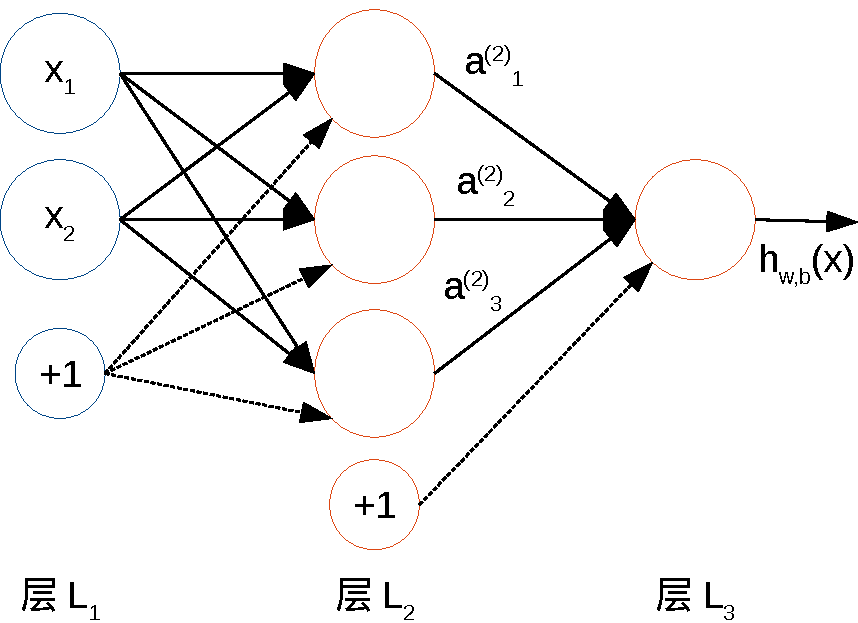
\includegraphics[width=0.9\textwidth]{image/illustration/network1.pdf}
				\caption{前馈神经网络模型示意图}
				\label{fig:lstm}
			\end{figure}
		\end{column}
	\end{columns}
}

\frame{
	\frametitle{卷积神经网络}
	\vspace{-0.8em}
	\begin{figure}
		\centering
		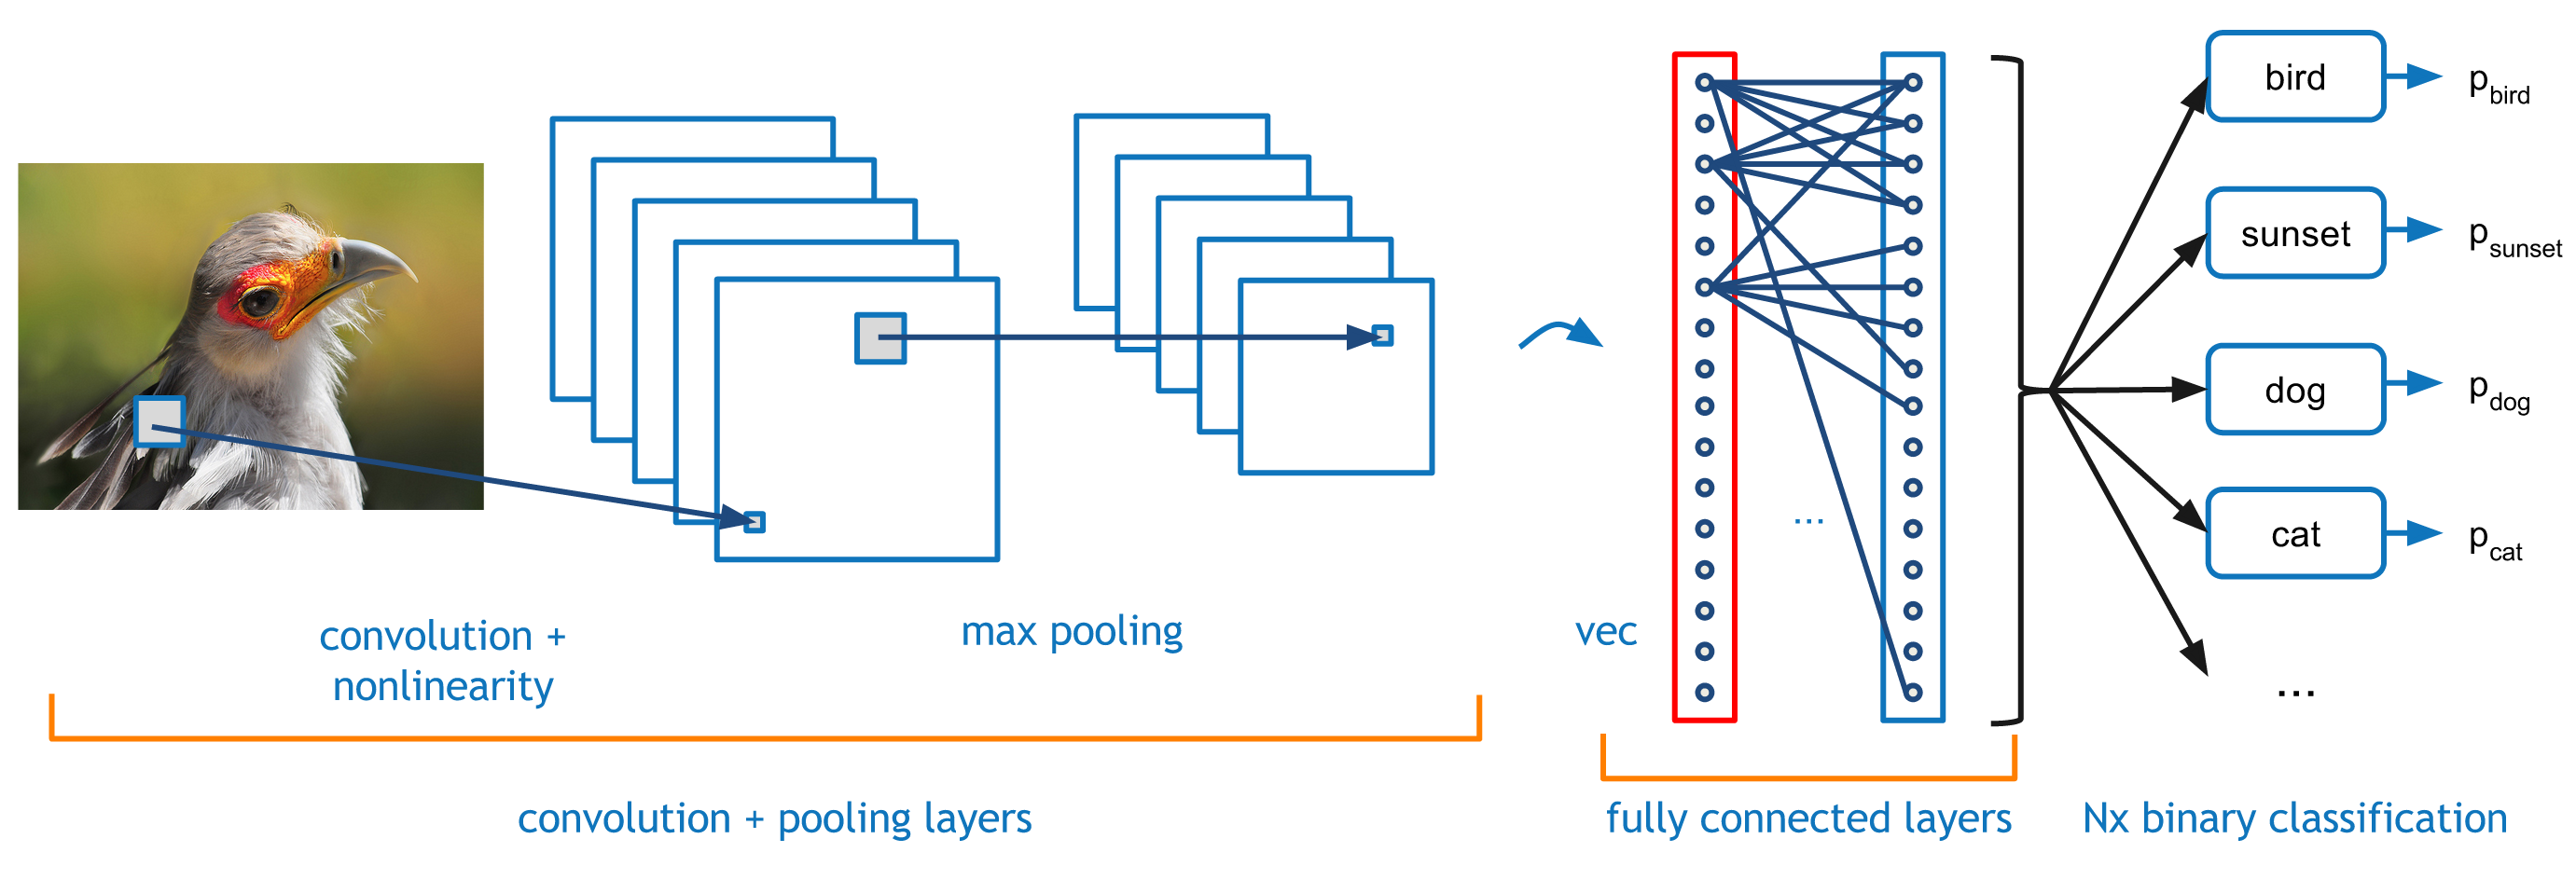
\includegraphics[width=0.8\textwidth]{figures/CNN}
		\caption{卷积网络模型示意图}
		\label{fig:network1}
	\end{figure}
	\vspace{-0.8em}
	\begin{block}{与前馈神经网络的区别}
		\begin{itemize}
			\item 直接作用于二维图像,无需特征设计阶段
			\item 卷积层,池化层
			\item 局部感知域,权重共享
		\end{itemize}
	\end{block}
}

\frame{
	\frametitle{长短记忆网络(处理一维信号)}
	\tiny
	\vspace{-2em}
	\begin{columns}[onlytextwidth]
		\begin{column}{0.5\textwidth}
			\begin{figure}[h] %structure of LSTM
				\centering
				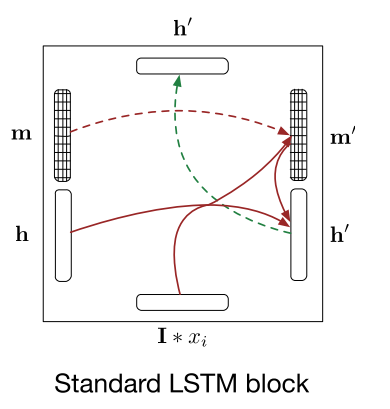
\includegraphics[width=0.6\textwidth]{figures/lstmblock1}
				\caption{长短记忆网络区块示意图}
				\label{fig:lstm}
			\end{figure}
		\end{column}
		%%%%%%% new column
		\begin{column}{0.5\textwidth}
			\begin{boxedminipage}{0.8\textwidth}
				\vspace{-1.5em}
				\begin{align}
					\label{eq:lstm}
					\begin{split}
						\textbf{g}^u &= \delta(\textbf{W}^u*\textbf{H}) \\
						\textbf{g}^f &= \delta(\textbf{W}^f*\textbf{H}) \\
						\textbf{g}^o &= \delta(\textbf{W}^o*\textbf{H}) \\
						\textbf{g}^c &= \mbox{tanh}(\textbf{W}^c*\textbf{H}) \\
						\textbf{m}' &= \textbf{g}^f \odot \textbf{m} + \textbf{g}^u \odot \textbf{g}^c \\
						\textbf{h}' &= \mbox{tanh}(\bf{g}^o \odot \bf{m}') \\
						\textbf{H} & = \begin{bmatrix}
							I*\textbf{x}_i \\ \textbf{h}
						\end{bmatrix}
					\end{split}
				\end{align}
			\end{boxedminipage}
		\end{column}
	\end{columns}

	\vspace{-1em}
	\begin{block}{缩写形式}
		\footnotesize
		\begin{equation*}
			(\textbf{h}', \textbf{m}') = \mbox{LSTM}\bigr(\textbf{H},\textbf{m},\textbf{W} \bigr)
		\end{equation*}
		其中\textbf{W}包含了四个门权值矩阵$\textbf{W}^u,\textbf{W}^f,\textbf{W}^o,\textbf{W}^c$。
	\end{block}
}

\frame{
	\frametitle{网格型长短记忆网络(处理N维信号)}
	\vspace{-1.5em}
	\begin{figure}[h]
		\centering
		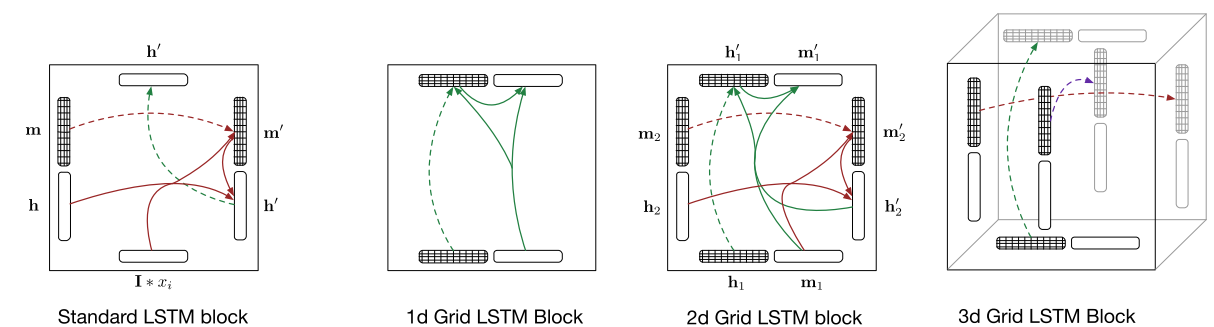
\includegraphics[width=\textwidth]{figures/gridlstm}
		\caption{网格型长短记忆网络区块示意图[Kalchbrenner et al, Grid LSTM, ICLR 2016]}
	\end{figure}
	\vspace{-2em}
	\begin{block}{网格型长短记忆网络更新过程}
		\tiny
		\begin{columns}[onlytextwidth]
			\begin{column}{0.4\textwidth}
				\vspace{-0.5em}
				\begin{equation}
					\textbf{H} = \begin{bmatrix}
						\textbf{h}_i \\ \vdots \\ \textbf{h}_N
					\end{bmatrix}
				\end{equation}
			\end{column}
			\begin{column}{0.6\textwidth}
				\vspace{-1em}
				\begin{align}
					\begin{split}
						(\textbf{h}_1', \textbf{m}_1') & =  \mbox{LSTM}(\textbf{H}, \textbf{m}_1, \textbf{W}_1) \\ &\mbox{ }\vdots \\
						(\textbf{h}_N', \textbf{m}_N') & =  \mbox{LSTM}(\textbf{H}, \textbf{m}_N, \textbf{W}_N)
					\end{split}
					\label{eq:gridlstm}
				\end{align}
			\end{column}
		\end{columns}
	\end{block}
}
\endinput
